\chapter{An Overview of Regular and Non-regular Solution}
\label{cha:overviewpart2}
% In PART I, we described the solution for both unconstrained and constrained problems in deep declarative nodes: its theoretical background of numerical optimization, the general solution for unconstrained and constrained optimization problems, and the details of the back-propagation in deep declarative noes. However, the solutions given before are based on the assumption of the existence of the solution and the second-order differentiable objective functions and constraints. In PART II, we will extend the solution for different non-regular solutions which can approximate the gradient of constrained problems. 
% \par In this chapter, we will give an overview of the non-regular point for deep declarative nodes with some related previous works. According to the definition of regular point in Definition~\ref{defn:regular-point}, we focus on the solution which is not regular, which means we cannot use the solutions we proposed in the previous chapter to solve them. 
% \par We first discuss possible non-regular solutions problems in the deep declarative nodes in Section~\ref{sec:problems-in-non-regular}, with corresponding specific examples. Next, we briefly discuss several previous related works in solving non-regular points problems in Section~\ref{sec:relatedworknonreg}. Since we set this chapter as the background information of our solutions in the next chapter, we also provide some comparison between these existed approaches. 
% \par We finally give a summary of the non-regular solution cases and our literature review findings. 


% \section{Problems in Regular Deep Declarative Nodes}
% \label{sec:problems-in-non-regular}

% \subsection{Assumptions and Problems}
% In Section~\ref{sec:bp}, we provided general solutions for unconstrained and constrained optimization problems in deep declarative nodes. For both problems, we assume that the solution of the problem, $y(x)$ exists in the neighborhood of the point $(x, y(x))$. Also, the objective function is supposed to be second-order differentiable. In particular, for constrained optimization problems, all constraints are also assumed to be second-order differentiable. These assumptions are made to guarantee that the optimal point is regular and strictly minimum. 
% \par However, not all problems have differentiable constraints and the jacobian or hessian matrix of constraints is full-ranked. Also, the first-order derivatives of the equality constraints and active inequality constraints may not linear independent. The dimension of the output may also various from the number of active constraints. According to the solution of equality constraints and inequality constraints in Equation~\ref{equ:solution-eq} and Equation~\ref{equ:solution-ineq} with their corresponding representations of matrix $H$, we have to compute the inverse of the matrix $H$ to get the solution. If $H$ is singular or very sparse, we are not able to get the exact solution since we cannot apply the Cholesky decomposition to this matrix. 
% \par There are many possible problems of non-regular solutions in the deep declarative nodes. We summarize them as three majority scenario: Overdetermined system, rank deficiency problems, and non-convex cases. 

% \subsection{Overdetermined System}
% If the constraints we get are more than unknowns we are going to solve, this system of equations is considered overdetermined. In declarative nodes, we require at least one degree of freedom for the back-propagation, since we have to update the gradient with the direction in a feasible solution set. Therefore, when the number of active constraints exceeds the dimensionality of the output, the system is overdetermined. 
% \begin{figure}[t]
%     \label{fig:overdetermined-solution}
%     \centering
%     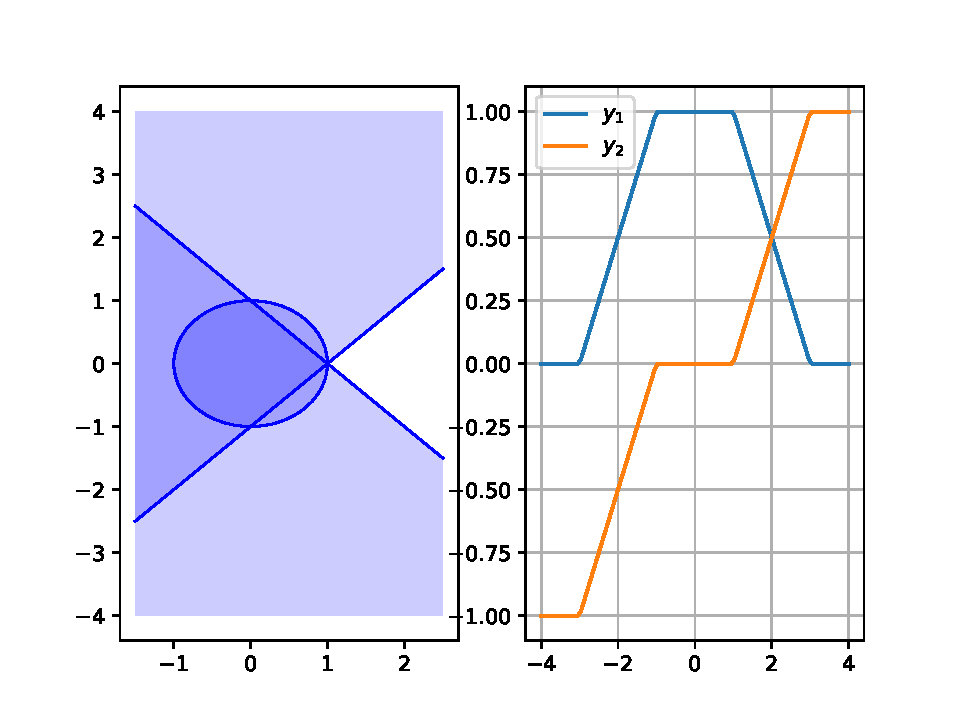
\includegraphics[page=1, width=.8\textwidth]{figs/overdetermined.pdf}
%     \caption{The feasible solution set and the results of the overdetermined system}
% \end{figure}
% \par We give the first example constrains the solution to a circle with two segments removed in Figure~\ref{fig:overdetermined-solution}. Also, we formulate this as the intersection of a (solid) circle constraint with two half-spaces. The problem is defined officially as 
% \begin{equation}
%     \begin{array}{llll}
%         y \in & \text{argmin}_u & \frac{1}{2} \|u - x\|^2 \\
%         & \text{subject to} & u_1^2 + u_2^2 - 1 \leq 0 & (h_1) \\
%         & & u_1 - u_2 - 1 \leq 0 & (h_2) \\
%         & & u_1 + u_2 - 1 \leq 0 & (h_3)
%     \end{array}
% \end{equation}
% From Figure~\ref{fig:overdetermined-solution}, there is only one intersection point among three constraints, where all three constraints are active. We calculate the graident of it using the implicit differentiation of the KKT optimality conditions as discussed in Equation~\ref{equ:solution-ineq} and their corresponding formulas. Figure~\ref{fig:overdetermined-gradient} shows the value of $y$ and the corresponding gradient. Using the solution for inequality constraints problems, we can get
% $$
% \begin{array}{llll}
%     A &= \text{D}_{Y} h(y) &= \begin{bmatrix}
%          2 y_1 & 2 y_2 \\ 1 & -1 \\ 1 & 1
%          \end{bmatrix} & \text{for active $h_i$} \\
%     B &= \text{D}^2_{XY} f(x, y) - \sum_{i=1}^{3} \lambda_i \text{D}^2_{XY} h_i(y) &= -I \\
%     C &= \text{D}_{Y} h(y) &= 0 \\
%     H &= \text{D}^2_{YY} f(x, y) - \sum_{i=1}^{3} \lambda_i \text{D}^2_{YY} h_i(y) &= (1 - 2 \lambda_1) I 
% \end{array}
% $$
% \begin{figure}[t]
%     \label{fig:overdetermined-gradient}
%     \centering
%     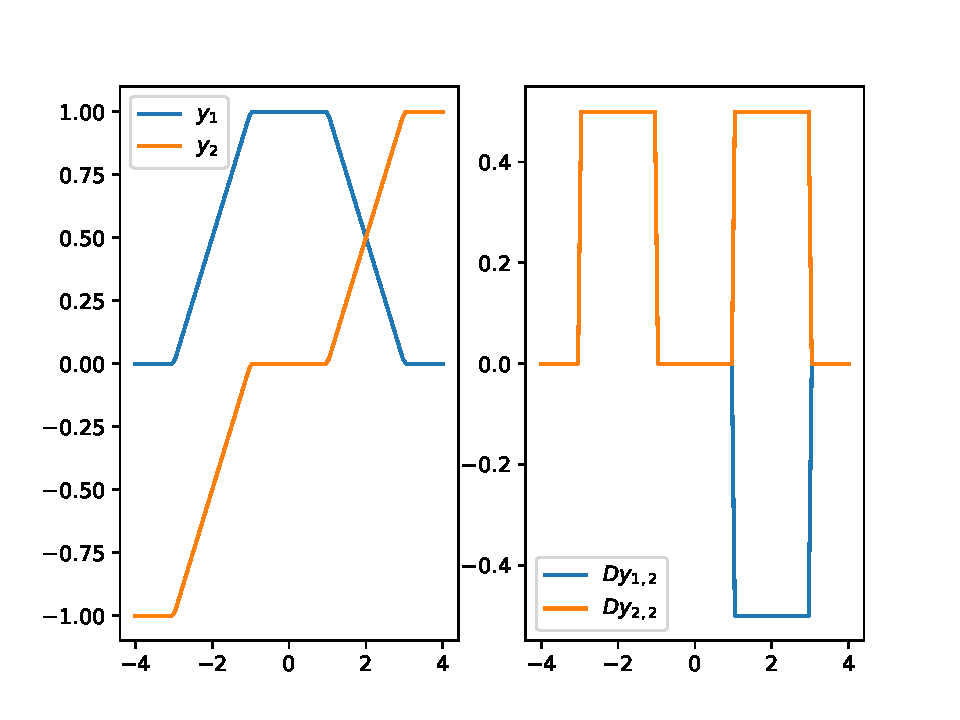
\includegraphics[page=1, width=.8\textwidth]{figs/overdetermined-gradient.pdf}
%     \caption{The results and corresponding gradient solution of the overdetermined system}
% \end{figure}
% where inactive constraints, and corresponding Lagrange multipliers, are first removed. Thus, the matrix $A$ may have between zero and three rows, which is not regular. This equation can be solved to give different results: 
% $$
% \text{D} y(x) = \begin{cases}
%         I & \text{if all constraints are inactive} \\
%         0 & \text{if all constraints are active (since $C = 0$)} \\
%         I - A^T (AA^T)^{-1} A & \text{if $h_1$ is inactive} \\
%         \frac{1}{1 - 2 \lambda_1} \left(I - A^T (AA^T)^{-1} A\right) & \text{otherwise.}
%     \end{cases}
% $$
% where the gradient is zero if all constraints are active. In this scenario, we can not perform back-propagation in our deep declarative network. 

% \subsection{Rank Deficiency Problems}
% Contrary to the overdetermined system, rank deficiency means that there are insufficient equations to determine the solution, which is the so-called underdetermined system. More generally, we do not have enough information to estimate the desired model in this case. 
% \par In declarative nodes, if the first-order derivatives of the equality constraints and active inequality constraints are linearly dependent, the solution points are not regular since the KKT conditions may still be satisfied but there are degrees of freedom in the Lagrange multipliers. The direct result is that matrix $H$ is sparse and singular. 
% \begin{figure}[t]
%     \label{fig:rank-deficiency}
%     \centering
%     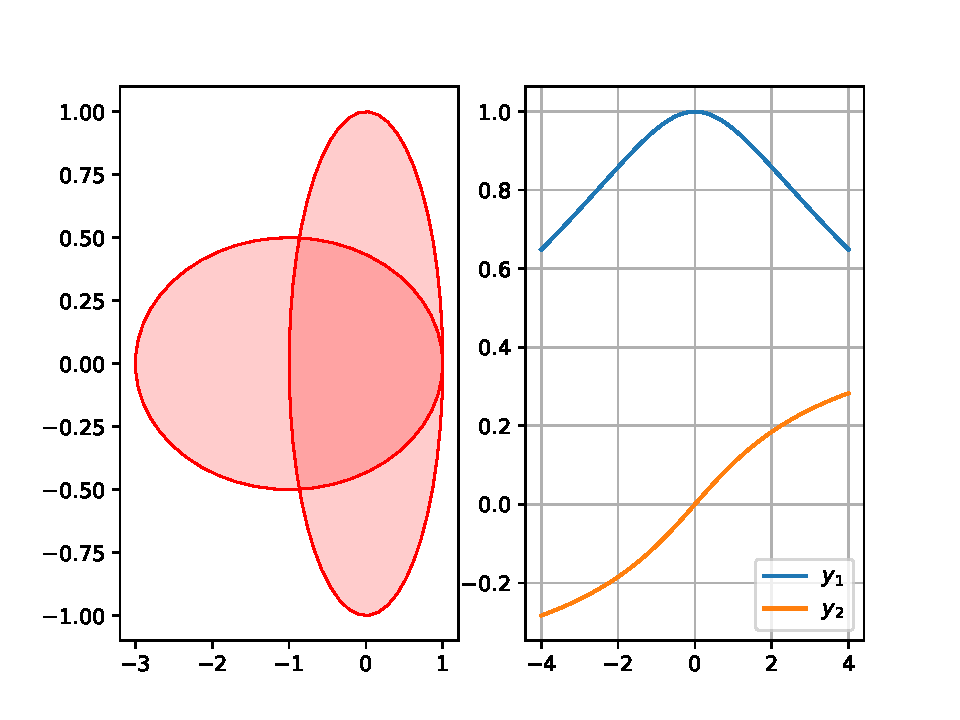
\includegraphics[page=1, width=.8\textwidth]{figs/rankdeficient.pdf}
%     \caption{The feasible solution set and the results of the rank-deficiency problem}
% \end{figure}
% \par We give the example that the constraint set is defined as the intersection between a circle and an ellipse in Figure~\ref{fig:rank-deficiency}. The problem is defined officially as
% \begin{equation}
%     \begin{array}{llll}
%         y \in & \text{argmin}_u & \frac{1}{2} \|u - x\|^2 \\
%         & \text{subject to} & u_1^2 + u_2^2 - 1 \leq 0 & (h_1) \\
%         & & \frac{1}{4}(u_1 + 1)^2 + 4 u_2^2 - 1 \leq 0 & (h_2)
%     \end{array}
% \end{equation}
% where the solution $y \in \mathbb{R}^2$ is a function of $x$ and at $x_2 = 0$, both constraints are active. This results in $A$ being rank deficient. 
% \par Similar to the previous overdetermined system, we can compute the gradient $\operatorname{D}y(x)$ of this rank deficient problem with each matrix as follows
% $$
% \begin{array}{lll}
%     A &= \begin{bmatrix}
%          2y_1 & 2 y_2 \\ \frac{1}{2} (y_1 + 1) & 8 y_2
%          \end{bmatrix} & \text{for active $h_i$} \\
%     B &= -I \\
%     C &= 0 \\
%     H &= \begin{bmatrix}
%          1 - 2 \lambda_1 - \frac{1}{2} \lambda_2 & 0 \\
%          0 & 1 - 2 \lambda_1 - 8 \lambda_2
%          \end{bmatrix}
% \end{array}
% $$
% where $A$ is rank deficient at $y = (1, 0)$. 

% \begin{figure}[t]
%     \label{fig:rank-deficiency-gradient}
%     \centering
%     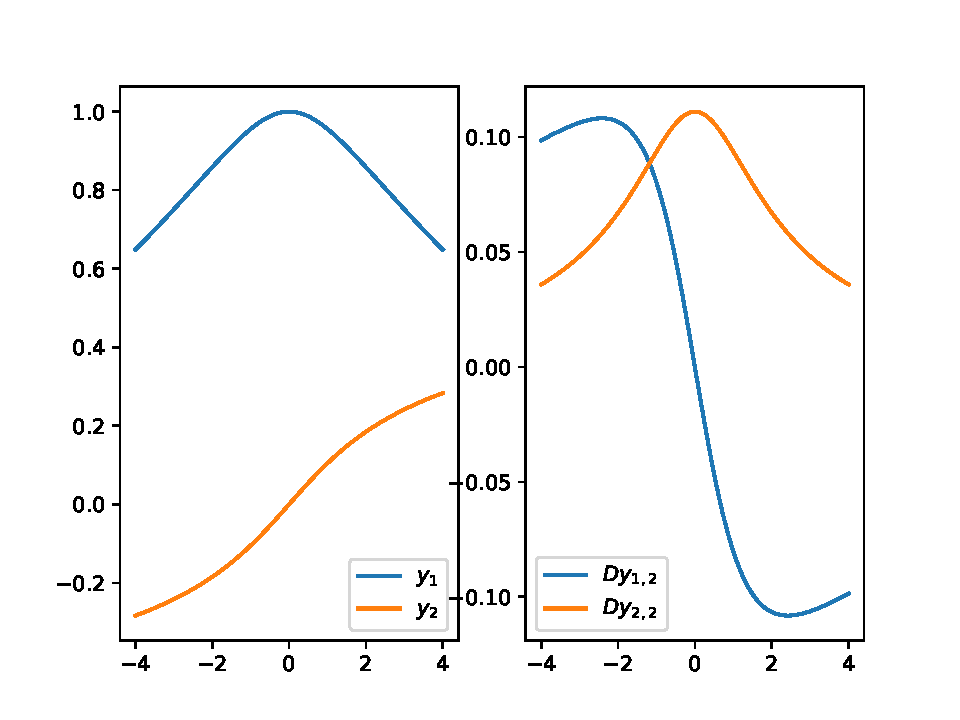
\includegraphics[page=1, width=.8\textwidth]{figs/gradient-rank-deficient.pdf}
%     \caption{The results and corresponding gradient solution of the rank-deficiency problem}
% \end{figure}
% \par Since in $A$, some columns are linear dependent, here we need to remove one of the rows of $A$ before solving for $\operatorname{D}y(x)$. One strategy is to keep those constraints where the rate of change of the objective is steepest relative to the curvature induced by the constraint surface. That is, remove from $A$ rows that are linearly dependent on other rows and with the smaller $\text{D}_{Y}f (\text{D}_{YY}^2 h_i)^{-1} \text{D}_{Y}f^T$. Figure~\ref{fig:rank-deficiency-gradient} shows the solution of $y$ with their corresponding gradient. 

% \subsection{Non-convex Cases}
% The last scenario is the non-convex cases, which is also a rank deficient problem. In general, solving a non-convex problem is NP-hard since it potentially has many local minima or solutions are in very flat regions, which is hard to update the gradient. 
% \par Similarly, we give the example that the constraint set is defined as the area in the circle that is not within the ellipse,
% \begin{equation}
%     \label{equ:non-convex}
%     \begin{array}{llll}
%         y \in & \text{argmin}_u & \frac{1}{2} \|u - x\|^2 \\
%         & \text{subject to} & u_1^2 + u_2^2 - 1 \leq 0 & (h_1) \\
%         & & \frac{1}{4}(u_1 + 1)^2 + 4 u_2^2 - 1 \geq 0 & (h_2)
%     \end{array}
% \end{equation}
% \begin{figure}[t]
%     \label{fig:non-convex}
%     \centering
%     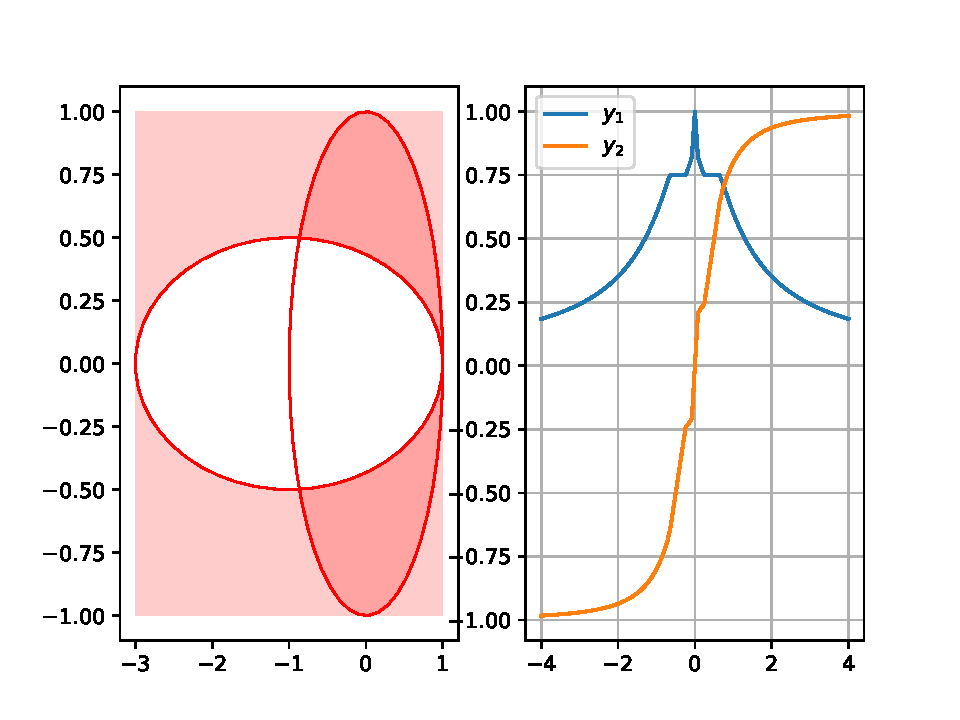
\includegraphics[page=1, width=.8\textwidth]{figs/nonconvex.pdf}
%     \caption{The feasible solution set and the results of the non-convex case}
% \end{figure}
% \par Figure~\ref{fig:non-convex} shows the feasible solution set, which is non-convex of this problem and the results $y$ with fixed $x_1 =0.75$ and $x_2$ sweeping from -4 to 4. When $x = (0.75, 0)$, the result $y = (1, 0)$ and both constraints $h_1$ and $h_2$ in Equation~\ref{equ:non-convex} are active. Thus at this point, the matrix $A$ is deficient.
% \begin{figure}[t]
%     \label{fig:non-convex-gradient}
%     \centering
%     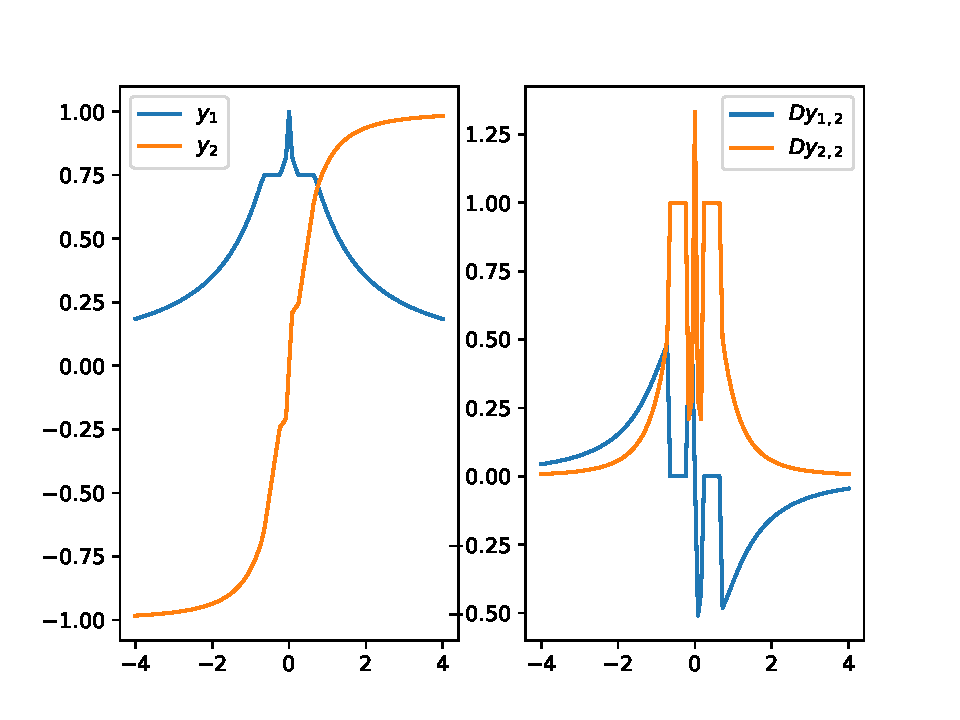
\includegraphics[page=1, width=.8\textwidth]{figs/gradient-non-convex.pdf}
%     \caption{The results and corresponding gradient solution of the non-convex case}
% \end{figure}
% \par Now we use the same method to calculate the gradient $\operatorname{D}y(x)$, we have
% $$
% \begin{array}{lll}
%     A &= \begin{bmatrix}
%          2y_1 & 2 y_2 \\ -\frac{1}{2} (y_1 + 1) & -8 y_2
%          \end{bmatrix} & \text{for active $h_i$} \\
%     B &= -I \\
%     C &= 0 \\
%     H &= \begin{bmatrix}
%          1 - 2 \lambda_1 + \frac{1}{2} \lambda_2 & 0 \\
%          0 & 1 - 2 \lambda_1 + 8 \lambda_2
%          \end{bmatrix}
% \end{array}
% $$
% where $A$ is rank deficient at $y = (1, 0)$. Figure~\ref{fig:non-convex-gradient} shows the solution of $y$ with their corresponding gradient. 
% \par We give an example for each non-regular solution scenario, which is not able to compute the gradient directly. In the next section, we discuss several previous related works in solving these problems. 

% \section{Related Work in Non-regular Solution}
% \label{sec:relatedworknonreg}
% Most previous works in the differentiable network only focus on the regular and convex solution. However, to some extent, dealing with non-regular solutions is solving non-regular linear systems. Therefore, we present several related works in discussing the solution of the overdetermined system, rank deficient problems, and non-convex cases in linear equations. Most of these approaches are based on theoretical optimization only, but some of them are problem-based, which means that in solving real computer vision tasks, we need to consider the actual problems then find the best solution. 
% \par \textbf{Overdetermined system.} The approximation of the solution for the overdetermined system is various. The most classical approach is the ordinary least squares, which minimize the $L_2$ residual between $Ax$ and $b$~\citep{AH:13}. However, if we want to have more numerical accurate solutions, QR factorization can give better results~\citep{TL:97}. Besides, \cite{BI:74} proposed the solution in the $L_1$ norm for calculating those data contains wild points, which are unstable with $L_2$ norm. They also introduced an algorithm to solve the linear Chebyshev data fitting problem, which is also overdetermined~\citep{BI:75}. Apart from them, \cite{WG:79} demonstrated a minimax solution for the overdetermined system of nonlinear equations based on the minimax norm. All these methods are similar since they are implemented to minimize the error between the exact solution and the approximation. 
% \par \textbf{Rank deficiency problems.} As an underdetermined system, many previous methods are provided through a similar approximation as the overdetermined system for the sparse matrix $A$. \cite{DD:05} demonstrated a method for finding the unique sparse solution by $L_1$ minimization and neighborliness of convex polytopes, which transferring the problem to a convex optimization problem. They also proved that the minimal $L_1$-norm solution is also the sparsest solution~\citep{DD:06}. Some other methods such as the successive overrelaxation method introducing the augmented coefficient matrix for finding the least square solution~\citep{DM:06} and transforming the matrix into a smaller full rank as sparse as possible one~\citep{WX:04} are also effective. Apart from the traditional methods, \cite{WJ:97} proposed an approach using recurrent neural networks to calculate the pseudoinverses of the rank deficient matrix, which is novel and practical. 
% \par \textbf{Non-convex cases.} Solving NP-hard problems directly is costly expensive. Actually, methods for solving convex optimization problems can also be applied to non-convex cases such as stochastic gradient descent~\citep{RH:51}, although the convergence is not guaranteed. Variance reduction is designed for nonconvex problems to improve the convergence of non-convex problems. \cite{RS:16} analyzed the stochastic variance reduced gradient method for non-convex problems, which achieved faster convergence than the traditional stochastic gradient method. \cite{AZ:16} also demonstrated an algorithm based on the variance reduction trick with the first-order minibatch stochastic
% method to accelerate the training. 

% \section{Summary}
% In Chapter~\ref{cha:overviewpart2}, we raise the problems from the original deep declarative nodes under the assumptions it makes. For these non-regular solution points, we discuss them in three scenarios: overdetermined system, rank deficient problems and non-convex cases, where the later two cases are underdetermined systems. All of these solutions are not able to compute the gradient directly since we cannot solve the linear system with traditional methods, and there is no exact solution. In addition, we introduce some related works in solving these irregular linear systems, which are approximating the closest solution to the problem by minimizing the residual norm. In the next chapter, for each scenario, we provide two efficient approaches and give a detailed comparison between these methods. 
